
%(BEGIN_QUESTION)
% Copyright 2009, Tony R. Kuphaldt, released under the Creative Commons Attribution License (v 1.0)
% This means you may do almost anything with this work of mine, so long as you give me proper credit

Calculate the differential pressure developed by an open venturi tube measuring air speed at 50 MPH, at sea level ($\rho_{air}$ = 0.00235 slugs/ft$^{3}$), where the throat diameter is one-half that of the entrance diameter:

$$\includegraphics[width=15.5cm]{i02984x01.eps}$$

Also, how much pressure will the venturi tube develop at twice the air speed (100 MPH)?

\underbar{file i02984}
%(END_QUESTION)





%(BEGIN_ANSWER)

$\Delta P$ at 50 MPH = 18.22 "W.C.

\vskip 10pt

$\Delta P$ at 100 MPH = 72.88 "W.C.

%(END_ANSWER)





%(BEGIN_NOTES)

%INDEX% Measurement, flow: venturi tube

%(END_NOTES)


